% TikZ and PGFPlots are not part of the engine's base TeX Live: they are
% fetched on demand from the package shelf the first time you compile, then
% cached in your browser for offline use.
\documentclass{article}
\usepackage[margin=2cm]{geometry}
\usepackage{tikz}
\usetikzlibrary{arrows.meta, positioning, shapes.geometric}
\usepackage{pgfplots}
\pgfplotsset{compat=1.17}

\begin{document}
\section*{A flowchart}
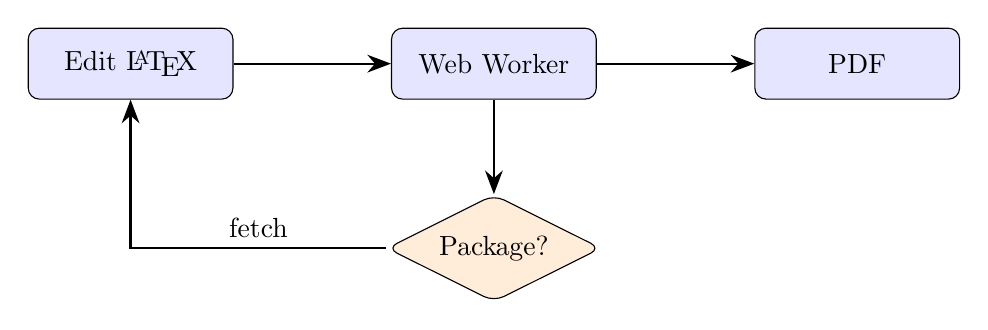
\begin{tikzpicture}[node distance=1.2cm and 2cm,
    box/.style={draw, rounded corners, fill=blue!10, minimum width=2.6cm, minimum height=0.9cm},
    arrow/.style={-{Stealth[length=3mm]}, thick}]
  \node[box] (edit) {Edit \LaTeX};
  \node[box, right=of edit] (worker) {Web Worker};
  \node[box, right=of worker] (pdf) {PDF};
  \node[box, below=of worker, diamond, aspect=2, fill=orange!15] (pkg) {Package?};
  \draw[arrow] (edit) -- (worker);
  \draw[arrow] (worker) -- (pdf);
  \draw[arrow] (worker) -- (pkg);
  \draw[arrow] (pkg.west) -| node[pos=0.25, above] {fetch} (edit.south);
\end{tikzpicture}

\section*{A plot}
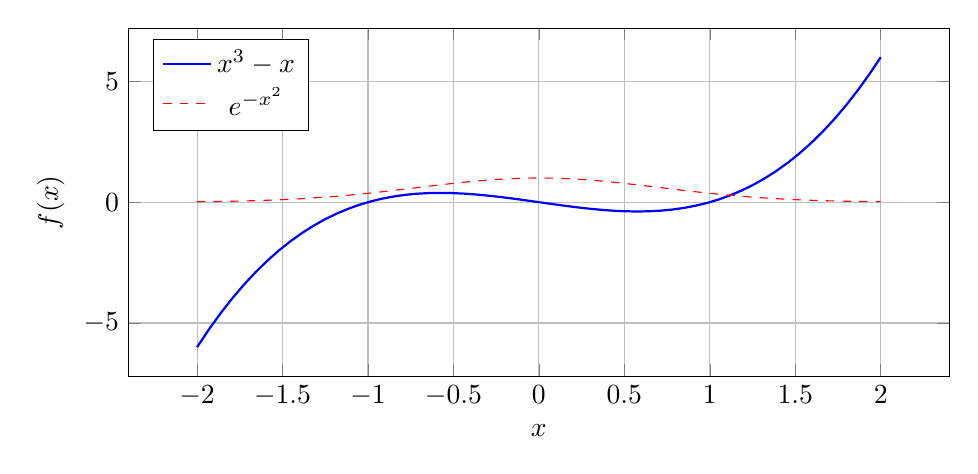
\begin{tikzpicture}
  \begin{axis}[width=12cm, height=6cm, grid=major, xlabel=$x$, ylabel=$f(x)$, legend pos=north west]
    \addplot[blue, thick, domain=-2:2, samples=60] {x^3 - x};
    \addlegendentry{$x^3 - x$}
    \addplot[red, dashed, domain=-2:2, samples=60] {exp(-x^2)};
    \addlegendentry{$e^{-x^2}$}
  \end{axis}
\end{tikzpicture}
\end{document}
